\documentclass[tikz,border=12pt]{standalone}
% Estilo comum dos esquemas vetoriais das aulas da GA033.
\usepackage[T1]{fontenc}
\usepackage[utf8]{inputenc}
\usepackage{lmodern}
\usepackage{amsmath,amssymb}
\usetikzlibrary{arrows.meta,positioning,calc,fit,matrix,decorations.pathreplacing,backgrounds,shapes.geometric}
\definecolor{lnccblue}{HTML}{075AC0}
\definecolor{ink}{HTML}{242A31}
\definecolor{muted}{HTML}{647080}
\definecolor{lightblue}{HTML}{EFF5FC}
\definecolor{teal}{HTML}{197C83}
\definecolor{orange}{HTML}{BC6A16}
\tikzset{
  every node/.style={font=\sffamily\fontsize{15}{18}\selectfont,text=ink},
  box/.style={draw=lnccblue,line width=0.9pt,fill=lightblue,inner sep=9pt,align=center},
  flow/.style={-{Stealth[length=3mm,width=2mm]},draw=lnccblue,line width=1pt},
  point/.style={circle,draw=lnccblue,fill=white,line width=1.2pt,minimum size=3.2mm,inner sep=0pt},
  label/.style={font=\sffamily\fontsize{13}{16}\selectfont,text=muted},
  heading/.style={font=\sffamily\bfseries\fontsize{16}{19}\selectfont,text=lnccblue}
}
% Impede setas horizontais involuntariamente invertidas após editar os nós.
\newdimen\origemseta
\newdimen\destinoseta
\newcommand{\verificarsetadireita}[2]{%
  \pgfextractx{\origemseta}{\pgfpointanchor{#1}{east}}%
  \pgfextractx{\destinoseta}{\pgfpointanchor{#2}{west}}%
  \advance\origemseta by 4mm%
  \ifdim\destinoseta>\origemseta\else
    \PackageError{diagramas}{Conector sem espaco entre #1 e #2}{Afaste os nos antes de compilar.}%
  \fi
}

\begin{document}
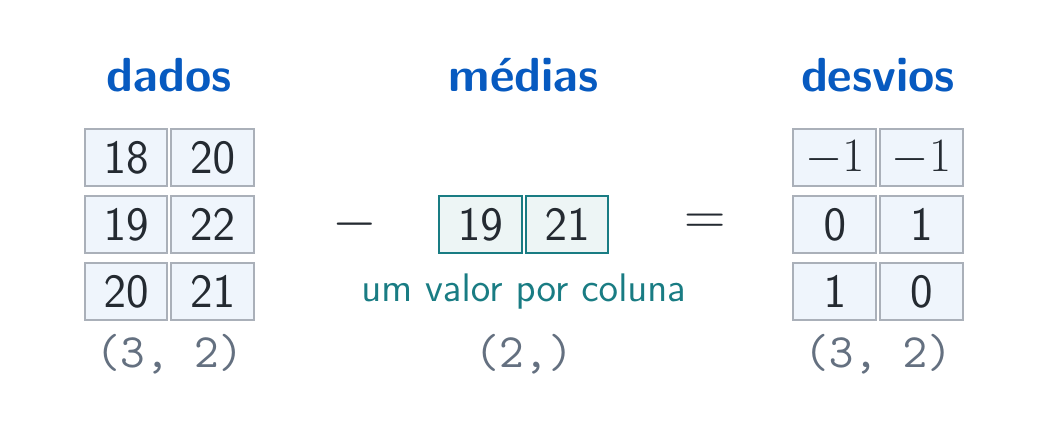
\begin{tikzpicture}[x=1cm,y=1cm,
  every node/.append style={font=\sffamily\fontsize{16}{19}\selectfont},
  cell/.style={draw=muted!55,line width=.7pt,minimum width=1.05cm,minimum height=.72cm,inner sep=0pt}]
  \path[use as bounding box] (0,0) rectangle (12.6,4.7);
  \node[heading] at (1.8,4.1) {dados};
  \node[heading] at (6.3,4.1) {médias};
  \node[heading] at (10.8,4.1) {desvios};
  \node[cell,fill=lightblue] at (1.25,3.05) {18};
  \node[cell,fill=lightblue] at (2.35,3.05) {20};
  \node[cell,fill=lightblue] at (1.25,2.2) {19};
  \node[cell,fill=lightblue] at (2.35,2.2) {22};
  \node[cell,fill=lightblue] at (1.25,1.35) {20};
  \node[cell,fill=lightblue] at (2.35,1.35) {21};
  \node[font=\sffamily\fontsize{22}{25}\selectfont] at (4.15,2.2) {$-$};
  \node[cell,draw=teal,fill=teal!8] at (5.75,2.2) {19};
  \node[cell,draw=teal,fill=teal!8] at (6.85,2.2) {21};
  \node[align=center,text=teal,font=\sffamily\fontsize{14}{17}\selectfont] at (6.3,1.35) {um valor por coluna};
  \node[font=\sffamily\fontsize{22}{25}\selectfont] at (8.6,2.2) {$=$};
  \node[cell,fill=lightblue] at (10.25,3.05) {$-1$};
  \node[cell,fill=lightblue] at (11.35,3.05) {$-1$};
  \node[cell,fill=lightblue] at (10.25,2.2) {0};
  \node[cell,fill=lightblue] at (11.35,2.2) {1};
  \node[cell,fill=lightblue] at (10.25,1.35) {1};
  \node[cell,fill=lightblue] at (11.35,1.35) {0};
  \node[text=muted] at (1.8,.55) {\texttt{(3, 2)}};
  \node[text=muted] at (6.3,.55) {\texttt{(2,)}};
  \node[text=muted] at (10.8,.55) {\texttt{(3, 2)}};
\end{tikzpicture}
\end{document}
